\section{Conclusions}
This work shows that it is possible to create a knowledge graph through 
semantic relationships, also known as ontological, that exist between objects 
that are usually found in interior spaces of human occupation, such as a room. 
In fact, the characterization occurs at the moment of defining the relationship 
that two objects have to each other, following the convention: 
\texttt{object1-predicate-object2}.

Thanks to Grakn it was possible to characterize objects, since through its 
high-level language it was possible to define the types of highly interconnected 
relationships between objects, since it provides a scheme that implements the 
principles of knowledge representation and reasoning.

It is important to highlight that this is an initial work that can be extended 
depending on the needs and requirements associated with the characterization 
of objects using knowledge graphs. Its utility was shown with the objects 
present in a room, but the spectrum can also be extended to an entire house, 
offices, or other closed and open spaces of human occupation.

On the other side, since an artificial intelligence project is made up of 
several parts (as much as needed), the knowledge graphs get involved in 
data acquisition phase and subsequently communicates with other 
systems that feed it back. This is important because the knowledge generated by 
the graph can serve as input to other models for object detection, such as 
convolutional neural networks or using YOLO systems.

As mentioned before, this work creates a semantic relationship of objects of an 
environment of human occupation given. This information could be useful for 
CNN models and could be added as an additional layer, called a 
``semantic layer''. This layer would work in conjunction with the CNN 
tagging phase, as shown in Figure \ref{fig:pipeline}.

\begin{figure}[H]
    \centering
    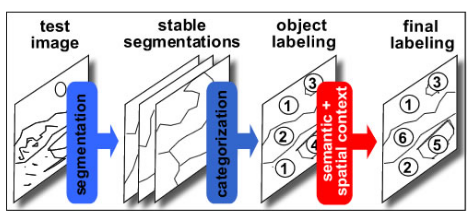
\includegraphics[width=6cm]{figures/pipeline.png}
    \caption{CNN generic pipeline model. Source \cite{Galleguillos2}}
    \label{fig:pipeline}
\end{figure}

Based on the results obtained, and given the utility of knowledge graphs 
in objects characterization, future work seeks to create and feed 
datasets, in JSON, XML or other formats, that contain ontological relationships 
of existing objects in a given indoor space of human occupation, such as a home, 
office and other places of rest or work. This will allow an understanding of 
the environment that surrounds users.

On the other side, we will seek to implement an improved version of the 
knowledge graph, in which new attributes are included, such as the 
\textit{probability of occurrence} between the relationship of two objects. 
For this approach, a previous dataset is required, from which we could count 
the relationships and then translate those data into probabilities.